% 默认页面大小 4:3
% \documentclass[10pt]{ctexbeamer}
% 页面大小 16:9
\documentclass[10pt, aspectratio=169]{ctexbeamer}


\usetheme{suep}

% 引入参考文献列表的 .bib 文件, 使用 GB/T 7714-2015 的文献著录规则.
\usepackage[backend=biber, style=gb7714-2015]{biblatex}
\addbibresource{ref.bib}

\usepackage{tipa}
\usepackage{xcolor}
\usepackage{fontawesome5}
\usepackage{unicode-math}
\usepackage{graphicx}
\usepackage{pdfpages}
\usepackage{hologo}
\usepackage{multicol}
\usepackage{booktabs}
\usepackage{fontspec}
\usepackage{bookmark}
\usepackage{minted}
\usepackage{hyperref}
\usepackage{cleveref}
\usepackage[font=small]{caption}
\usepackage{tikz}
\usepackage{algorithm2e}

\renewcommand{\thefigure}{\Roman{figure}}

\setCJKmainfont[
  Path=fonts/,
  Extension=.otf,
  UprightFont=SourceHanSerifSC-SemiBold,
  BoldFont=SourceHanSerifSC-Heavy,
  ItalicFont=SourceHanSerifSC-SemiBold,
  BoldItalicFont=SourceHanSerifSC-SemiBold
]{SourceHanSerifSC-Regular}

% 定义一些特殊的command

\def\rawcmd#1{\texttt{\color{blue}\footnotesize #1}}
\newcommand\pkg[1]{\texttt{#1}}
\newcommand\link[1]{\href{#1}{\faLink}}
\definecolor{LightGray}{gray}{0.9}

% 开始文档 *****************************************************************

\title{ \LaTeX{} 排版简要介绍 }
\subtitle{从入门到放弃}
\author[Haiwen\,Zhang]{\href{mailto:haiwen.zhang@zju.edu.cn}{纸上得来终觉浅}}
\institute{数理学院数学系}
\date[\today]{\today, 中国上海}
\subject{展示主题}
\keywords{展示, 关键词}

\begin{document}

\begin{frame}[plain]
  \maketitle
\end{frame}

\begin{frame}[t]
  \frametitle{目录}
  \tableofcontents
\end{frame}

\section{介绍}

\begin{frame}{先声夺人}
  \centering
  \scalebox{5}{\textipa{/"leItEk/}}
\end{frame}

\begin{frame}{\LaTeX{} 是什么?\mbox{}——\mbox{}你为什么学}
\pause
\begin{itemize}
  \item<+-> Word 替代品?

    \begin{itemize}
      \item 「我受够了,我以后什么都要用 \LaTeX{} 写」
    \end{itemize}

  \item<+-> 写论文神器?

    \begin{itemize}
      \item 「我就是为大 paper 而生的,当然必须学 \LaTeX{} 啦」
    \end{itemize}

  \item<+-> 打公式方便?

    \begin{itemize}
      \item 「复杂公式输入哪家强,当然首选 \LaTeX{} 帮忙」
    \end{itemize}
\end{itemize}
\end{frame}


\begin{frame}[fragile]
\frametitle{\LaTeX{} 是什么?\mbox{}——\mbox{}What you \emph{think} is what you get!}
\begin{columns}
\begin{column}{0.48\textwidth}
  \centering
  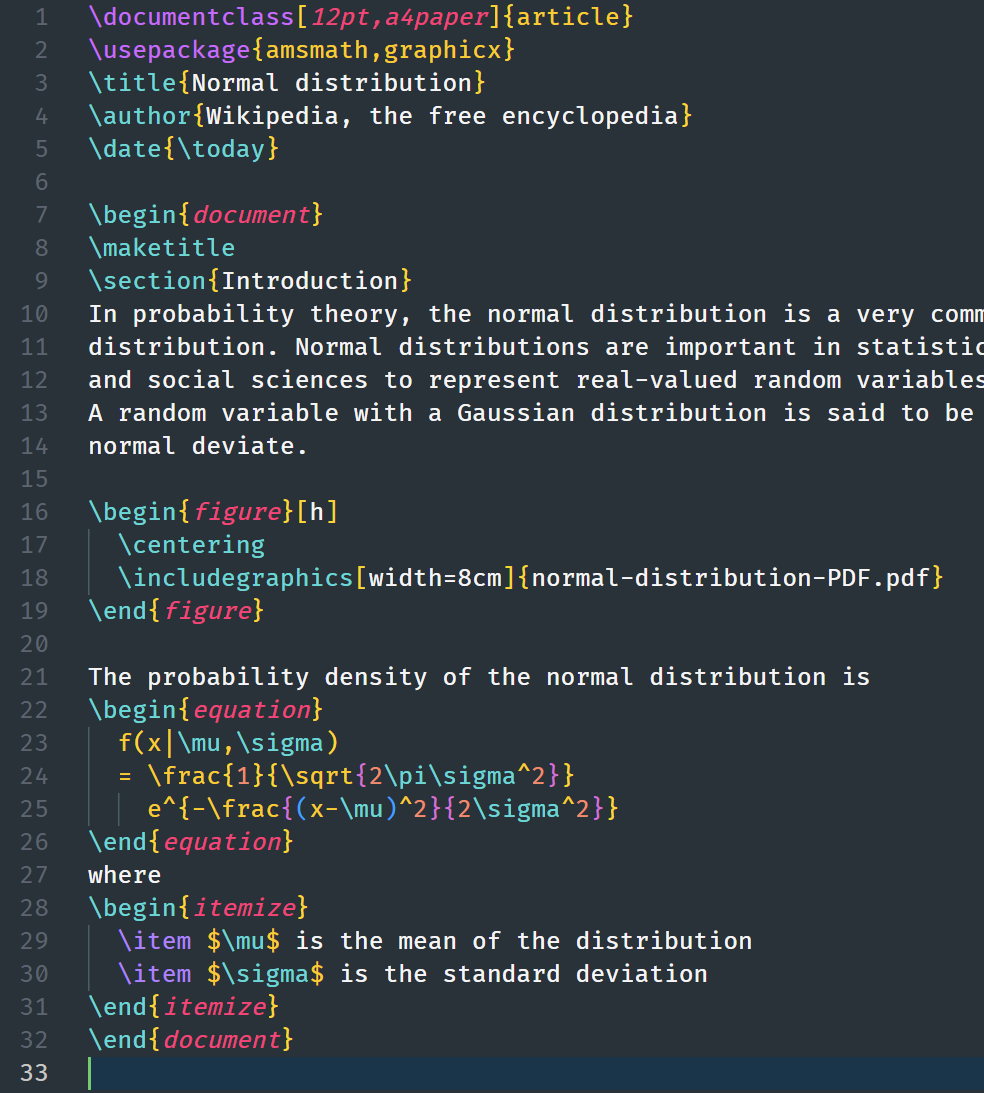
\includegraphics[width=0.75\textwidth]{images/code.png}
\end{column}
\begin{column}{0.48\textwidth}
  \begin{figure}
    \centering
    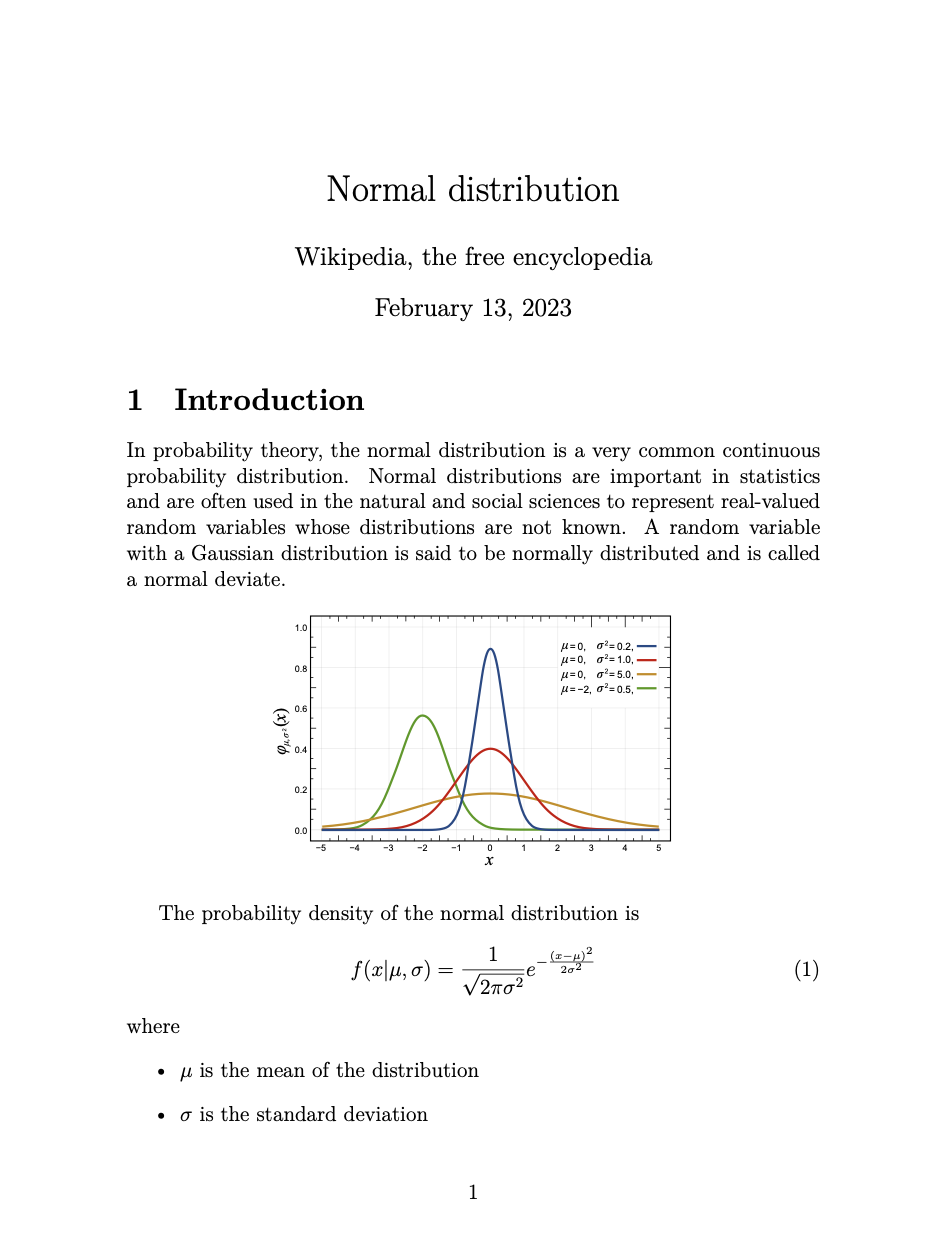
\includegraphics[width=0.75\textwidth]{images/normal-dist.png}
  \end{figure}
\end{column}
\end{columns}
\end{frame}

\begin{frame}{基本原则}
  \begin{itemize}
    \item<+-> 排版 vs 文字处理

      \begin{itemize}
        \item 《别把 \LaTeX{} 当 Word 用》
        \item {\scriptsize 在固定版面内,摆置各种不同类型的资料,以最合适的方法呈现 \href{https://zh.wikipedia.org/wiki/排版}{\faWikipediaW}}
      \end{itemize}

    \item<+-> 遵循业界规范
    \item<+-> 追求良好的阅读体验 (readability)
    \item<+-> 内容与格式分离
    \item<+-> \alert{内容永远比格式重要!}
  \end{itemize}
\end{frame}

\subsection{\TeX 排版系统历史}

\begin{frame}[fragile]{\TeX 与 \LaTeX{} 的起源}
  \begin{columns}[T]
    \column{.7\textwidth}
    \begin{itemize}
      \item \TeX: $\tau\varepsilon\chi$ (\textipa{/'tEx/},
        \textipa{/'tEk/})
        \begin{itemize}
          \item 生成精美图书的排版系统
          \item 最初由 高德纳\footnote{1974年图灵奖得主,《计算机程序设计艺术》(The Art of Computer Programming)作者。} (Donald E.~Knuth) 于 1978 年开发  
          \item 最新版本为 \TeX\ 3.14159265
          \item 漂亮、美观、稳定、通用
          \item 尤其擅长数学公式排版
        \end{itemize}

        \vspace{2em}
      \item \LaTeX{}(\textipa{/'la:tEx/}, \textipa{/'leItEk/})
        \begin{itemize}
          \item Leslie Lamport\footnote{2013年图灵奖得主,对于分布式及并形系统的理论与实践具有基础性贡献。} 开发的一种 \TeX 格式
          \item 在 \TeX 的基础上提供宏包, 降低使用门槛
          \item 极其丰富的宏包,提供扩展功能
          \item 广泛用于学术界,期刊会议论文模板
        \end{itemize}
    \end{itemize}
    \column{.2\textwidth}
    \vspace*{-5mm}
    \hspace{-10mm} 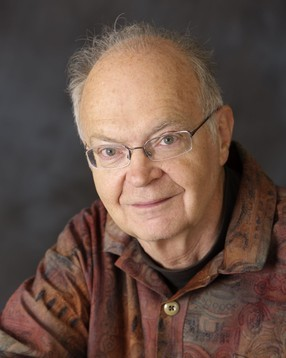
\includegraphics[width=\textwidth]{images/Knuth.jpg}

    % \vspace*{5mm}
    \hspace{-10mm} 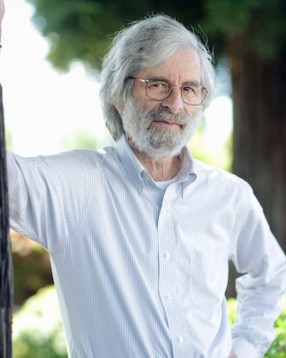
\includegraphics[width=\textwidth]{images/Lamport.jpg}

  \end{columns}
\end{frame}

\subsection{\LaTeX{} 利弊}

\begin{frame}[fragile]{\LaTeX{} 的好处与坏处}
    \textbf{好处}
    \begin{itemize}
        \item 数学公式排版优雅 \quad $\mathcal{F}(\xi)=\int_{-\infty}^{\infty} f(x)\mathrm{e}^{-\mathrm{j}2\pi \xi x}\,\mathrm{d}x$
        \item 内容与格式分离
        \item 随心所欲的宏定义与自定义命令 \rawcmd{\textbackslash newcommand},\rawcmd{\textbackslash def}
    \end{itemize}

    \pause

    \vspace{2em}
    \textbf{坏处}
    \begin{itemize}
        \item 得到易读的版本,需要编译
        \item 输入相对 Word 繁琐
        \item 非开箱即用。有时自行解决编辑器、宏包,甚至是编译错误。
    \end{itemize}

\end{frame}

\section{\LaTeX{} 安装}

\begin{frame}{选择发行版}
    \begin{itemize}
    \item \TeX{} 发行版distribution

        \begin{itemize}
        \item 引擎、宏包、字体、文档的综合体
        \item 类比 Visual Studio
        \item \TeX{} Live、Mac\TeX{}、W32\TeX{}、MiK\TeX{} 等
        \end{itemize} \pause

    \item \TeX{} Live \link{https://www.tug.org/texlive}

        \begin{itemize}
        \item 官方维护,首选,跨平台
        \item Mac\TeX{} ≈ macOS 下的 \TeX{} Live
        \item 缺点:完整版体积大7GB+、每年需重装
        \end{itemize}

    \item MiK\TeX{} \link{https://miktex.org}

        \begin{itemize}
        \item 由 Christian Schenk 维护(是个狠人)
        \item 宏包随用随装
        \item 缺点:部分细节与 \TeX{} Live 不兼容、网络问题
        \end{itemize} \pause

    \item \alert{不要安装 \CTeX{} 套装!}

        \begin{itemize}
        \item \alert{存在严重 bug,并且完全过时(2012年已经停止维护)。}
        \end{itemize}
    \end{itemize}
\end{frame}


\begin{frame}{选择本地编辑器}
  LaTeX 也是纯文本文件,后缀名为 .tex,可以用任何文本编辑器编写

    \begin{itemize}
      \item<+-> 专用型
    
        \begin{itemize}
          \item TeXworks:\TeX{} Live 自带 \faWindows{} \faApple{} \faLinux{}
          \item \emph{TeXStudio}:功能丰富,对新手友好 \faWindows{} \faApple{} \faLinux{}
          \item TeXShop:Mac\TeX{} 自带 \faApple{}
          \item WinEdt:功能丰富,收费 \faWindows{}
        \end{itemize}
    
      \item<+-> 通用型
    
        \begin{itemize}
          \item \emph{Visual Studio Code}:借助插件 \pkg{LaTeX Workshop} + \pkg{LaTeX Utilities}
          \item Sublime Text:收费
          \item Vim:q、q!、wq、wq!、...???
          \item Emacs:ctrl-s、ctrl-c ctrl-x、...???
        \end{itemize}

    \end{itemize}
\end{frame}

\begin{frame}{不想安装?}
  \begin{itemize}
  \item 云端服务更好用…吗?
  \item 免去安装、升级等一系列烦恼,可以多人协作
  \item 版本控制、模板市场
  \end{itemize} \pause

  \begin{itemize} \small
  \item Overleaf:
      \href{https://cn.overleaf.com}{\textcolor[HTML]{138a07}{Overleaf} \faLink}

      \begin{itemize}
      \item 模板丰富
      \item 用户支持很好
      \pause
      \item 注意网络环境(咳咳)
      \end{itemize}
  \end{itemize}

\end{frame}

\begin{frame}{引擎}
  \begin{itemize}
    \item 引擎即编译器,是编译源代码生成文档的排版引擎
      \begin{itemize}
        \item 有 TeX、pdfTeX、XeTeX、LuaTeX 等
      \end{itemize}
    \item 有两种语言的格式,分别为 plainTeX(最初版本)和 LaTeX
    \item 编译指令即编译源代码生成文档的命令,根据引擎和格式来选择
    \begin{table}[]
      \begin{tabular}{|c|c|c|c|}
      \hline
       引擎 & 目标格式 & 使用plainTex  & 使用 LaTeX  \\ \hline
       TeX & DVI & tex &  \\ \hline
       pdfTeX & DVI & etex &  latex \\ \hline
       pdfTeX & PDF & pdftex & 	pdflatex \\ \hline
       XeTeX & PDF & xetex & xelatex \\ \hline
       LuaTeX & PDF & luatex & lualatex \\ \hline
      \end{tabular}
    \end{table}
  \end{itemize}
\end{frame}

\begin{frame}{编译指令}
  \begin{itemize}
    \item 纯文本文件,后缀名为 \texttt{.tex}(类比 Markdown 的 \texttt{.md})
    \pause
    \item 选择正确的编译指令
        \begin{itemize}
            \item 例如 \texttt{xelatex main.tex}
            \item 文中含有交叉引用、参考文献、目录等情况,需要多次编译
            \item \texttt{latexmk} 秒了
        \end{itemize}
    \pause
    \item VSCode:LaTeX Workshop 插件秒了
    \item Overleaf 秒了
  \end{itemize}
\end{frame}


\begin{frame}{推荐安装}
    \begin{itemize}
      \item<+-> 本地版最佳实践
    
        \begin{itemize}
            \item + MiK\TeX{}
            \item + Visual Studio Code (LaTeX Workshop 等插件)
            \item + git(代码管理工具)
            \item + Github(全世界最大的程序员交友网站)
        \end{itemize}
      
      \item<+-> 网络版最佳实践
        \begin{itemize}
          \item 在线编辑器 \href{https://cn.overleaf.com}{\textcolor[HTML]{138a07}{Overleaf} \faLink} 编写
        \end{itemize}

      \item<+-> \href{https://suepaper.github.io/math201/docs/latex/}{\textcolor[HTML]{138a07}{保姆级手把手的教程} \faLink}

    \end{itemize}
\end{frame}


\section{Hello world案例}

\begin{frame}[fragile]{Hello World!}
  \begin{minted}
    [
      frame=lines,
      framesep=2mm,
      baselinestretch=1.2,
      bgcolor=LightGray,
    ]{tex}
% 用 pdfLaTeX、XeLaTeX 或 LuaLaTeX 编译
\documentclass{article}
\begin{document}
Hello world!
\end{document}
  \end{minted}
  \pause
  \begin{minted}
  [
    frame=lines,
    framesep=2mm,
    baselinestretch=1.2,
    bgcolor=LightGray,
  ]{tex}
% 用 XeLaTeX 或 LuaLaTeX 编译
\documentclass{ctexart}
\begin{document}
你好中国!
\end{document}
  \end{minted}
\end{frame}

\begin{frame}{语法}
  \begin{itemize}
      \item 命令(控制序列):以 \texttt{\textbackslash} 开头,大小写敏感
      \begin{itemize}
          \item \mintinline{tex}{\LaTeX{}} $\to$ \LaTeX{}
          \item 有作用域的概念,可以用 \texttt{\{\}} 限定作用域
          \item 可以接收参数,如 \mintinline{tex}{\documentclass{book}}
          \item 必需参数用 \texttt{\{\}},可选参数用 \texttt{[]}
      \end{itemize} 
      \pause
      \item 注释以 \texttt{\%} 开头
      \item 连续多个空格 = 单个空格 = 单个换行
      \item 可以定义自己的命令
  \end{itemize}
\end{frame}

\section{填写创作}

\begin{frame}[fragile]{文件的结构}
  \begin{minted}
    [
      frame=lines,
      framesep=2mm,
      baselinestretch=1.2,
      bgcolor=LightGray,
    ]{tex}
  \documentclass{article} % 文档类
  % 导言区 (preamble):加载宏包、定义命令、设置文档格式等
  
  \begin{document}        % 文档开始
  % 正文区 (body):文档的内容
  Hello world!
  \input{content.tex}     % 也可以导入其他文件内容
  \end{document}          % 文档结束,后续内容不会被编译
  \end{minted}
\end{frame}

\begin{frame}[fragile]{文档类与宏包}
  \begin{itemize}
      \item \LaTeX{} 文档开头必须包含 \mintinline{tex}{\documentclass} 指定文档类
      \item 基础文档类:\texttt{article}、\texttt{report}、\texttt{book}、\texttt{beamer} 等
      \item 中文变体:\texttt{ctexart}、\texttt{ctexrep}、\texttt{ctexbook}、\texttt{ctexbeamer} 等
      \item 可以通过可选参数指定字号、纸张大小、双面打印等选项
      \begin{minted}{tex}
          \documentclass[12pt, a4paper, twoside]{article}
      \end{minted}
      \pause
      \item 宏包相当于第三方库,可以引入更丰富的扩展功能
      \begin{minted}{tex}
          \usepackage{amsmath}
          \usepackage[final]{minted}
      \end{minted}
      \item \TeX{} Live full 自带大量宏包
      \item 通过 \texttt{texdoc \textit{package}} 查看文档
  \end{itemize}
\end{frame}

\section{段落及排版样式}

\begin{frame}[fragile]{段落 (paragraph)}
  \begin{itemize}
      \item 正常写作即可,以空行或 \mintinline{tex}{\par} 分段
      \item 行首空格会被忽略,多个空格会被合并为一个
      \item 换行在非中文语境下视作一个空格
  \end{itemize}
  
  \vspace{1em}
  \pause
  \begin{columns}
      \begin{column}{0.5\textwidth}
          \begin{minted}[frame=lines,framesep=2mm,baselinestretch=1.2,bgcolor=LightGray,fontsize=\scriptsize]{tex}
Consecutive spaces    are
squashed     in \LaTeX{}. 中文语境下
不会添加空格。Leading spaces are
    ignored. Trailing comment does%
n't break a word.

A new paragraph.\par
或者用 \verb|\par| 也可以。
          \end{minted}
      \end{column}
      \begin{column}{0.45\textwidth}
          \setlength{\parskip}{.5em}\small
  Consecutive spaces    are
  squashed     in \LaTeX{}. 中文语境下
  不会添加空格。Leading spaces are
      ignored. Trailing comment does%
  n't break a word.
  
  A new paragraph.\par
  或者用 \verb|\par| 也可以。
      \end{column}
  \end{columns}
\end{frame}
  
\begin{frame}[fragile]{断行与断页}
\begin{itemize}
    \item 可以用 \mintinline{tex}{\\} 或 \mintinline{tex}{\newline} 强制断行
    \begin{itemize}
        \item 类似 Word 中的``软回车'',不会产生新的段落
    \end{itemize}
    \item \mintinline{tex}{\newpage} 强制断页
    \item \mintinline{tex}{\clearpage} 强制断页并清空\emph{浮动体}
    \begin{itemize}
        \item We'll cover this soon ;)
        \item 一般用 \mintinline{tex}{\newpage} 即可
    \end{itemize}
\end{itemize}
\vspace{1em}
\pause

\begin{columns}
    \begin{column}{0.5\textwidth}
        \begin{minted}[frame=lines,framesep=2mm,baselinestretch=1.2,bgcolor=LightGray,fontsize=\scriptsize]{tex}
Starting a new paragraph. \\
Oops, a new line within it.

Finally another paragraph. \newline
Another new line, oh my!
        \end{minted}
    \end{column}
    \begin{column}{0.45\textwidth}
        \setlength{\parskip}{.5em}\small
Starting a new paragraph. \\
Oops, a new line within it.

Finally another paragraph. \newline
Another new line, oh my!
    \end{column}
\end{columns}
\end{frame}
  
\begin{frame}[fragile]{字形与字号}
\begin{itemize}
    \item 有两类修改字形的命令:\\\mintinline{tex}{{\bfseries bold}} 和 \mintinline{tex}{\textbf{bold}}
    \begin{itemize}
        \item 前者对作用域内的所有内容生效,后者只对参数内容生效
        \item 都是“内置”字体的不同样式,自定义字体?留作习题
    \end{itemize}
    \item 修改字号:\mintinline{tex}{{\large Hi}}
    \item \alert{汉字一般不使用斜体}
    \pause
    \item \alert{不要滥用字体样式}{\scriptsize(本页除外)} 
\end{itemize}
\pause
\begin{columns}
    \begin{column}{0.62\textwidth}
        \begin{minted}[frame=lines,framesep=2mm,baselinestretch=1.2,bgcolor=LightGray,fontsize=\scriptsize]{tex}
\textbf{bold} \textsf{sans serif}
\texttt{typewriter} \textsc{Small Caps}
\textit{italic} \textsl{slanted}

{\tiny tiny} {\scriptsize scriptsize}
{\footnotesize footnotesize} {\small small}
{\normalsize normalsize} {\large large}
{\Large Large} {\LARGE LARGE}
{\huge huge} {\Huge Huge}
        \end{minted}
    \end{column}
    \begin{column}{0.39\textwidth}\vspace{-2em}

\textbf{bold} \textsf{sans serif}
\texttt{typewriter} \textsc{Small Caps}
\textit{italic} {\addfontfeatures{AutoFakeSlant}\textsl{slanted}}

{\tiny tiny} {\scriptsize scriptsize}
{\footnotesize footnotesize} {\small small}
{\normalsize normalsize} {\large large}
{\Large Large} {\LARGE LARGE}
{\huge huge} {\Huge Huge}
    \end{column}
\end{columns}
\end{frame}
  
\begin{frame}[fragile]{关于字符和标点}
\begin{itemize}
    \item 特殊字符需要转义,如 \mintinline{tex}{\_}、\mintinline{tex}{\%}、\mintinline{tex}{\$}、\mintinline{tex}{\&}、\mintinline{tex}|\{|、\mintinline{tex}|\}| 等等
    \begin{itemize}
        \item \mintinline{tex}{\~{}}、\mintinline{tex}{\^{}} 带大括号防止将后面的字符理解为参数
        \item \mintinline{tex}{\textbackslash} 反斜杠
    \end{itemize}
    \item 西文语境下的引号:\mintinline{tex}{``double''} \quad ``double''
    \begin{itemize}
        \item 中文语境下正常输入即可
    \end{itemize}
    \item 连字符:\mintinline{tex}{-}、短破折号:\mintinline{tex}{--}、长破折号:\mintinline{tex}{---}
    \begin{itemize}
        \item Newton-Leibniz Formula
        \item Henry Kissinger (1923--2023)
        \item Don't use \texttt{\$\$} --- it breaks spacing!
    \end{itemize}
    \item 防止西文连字:\mintinline{tex}{dif{}f{}icult} \quad dif{}f{}icult
    \begin{itemize}
        \item 对比:difficult
    \end{itemize}
\end{itemize}
\end{frame}
  
\begin{frame}[fragile]{强制行距/间距}
\begin{itemize}
    \item 长度单位:pt,in(英寸),cm,mm,em(小写 `m' 的宽度),ex(小写 `x' 的高度)
    \item 行距:\mintinline{tex}{\linespread{factor}}(默认行距 1.2 倍字号大小)
        \begin{itemize}
            \item 局部修改要在后面加 \mintinline{tex}{\selectfont},且要在范围内手动分段
        \end{itemize}
    \item 插入水平间距(多空格无效):\mintinline{tex}{\hspace{length}}
        \begin{itemize}
            \item \mintinline{tex}{\quad} 相当于 1em,\mintinline{tex}{\qquad} 相当于 2em
            \item \mintinline{tex}{\hspace*} 防止因为断行而消失
        \end{itemize}
    \item 插入垂直间距:\mintinline{tex}{\vspace{length}}
        \begin{itemize}
            \item \mintinline{tex}{\\[1em]} 可以在换行的同时插入垂直间距
        \end{itemize}
\end{itemize}
\pause
\begin{columns}
    \begin{column}{0.5\textwidth}
        \begin{minted}[frame=lines,framesep=2mm,baselinestretch=1.2,bgcolor=LightGray,fontsize=\tiny]{tex}
{\linespread{1.6}\selectfont This is a paragraph with 1.6 linespread.\\
This is the next line and \quad space and \hspace{3em} more and
\hspace{\fill}lol\par}

\vspace{-1em}Next paragraph.\\[1em] and next line.
        \end{minted}
    \end{column}
    \begin{column}{0.45\textwidth}
        \setlength{\parskip}{.5em}\scriptsize
{\linespread{1.6}\selectfont This is a paragraph with 1.6 linespread.\\
This is the next line and \quad space and \hspace{3em} more and
\hspace{\fill}lol\par}

\vspace{-1em}Next paragraph.\\[1em] and next line.
    \end{column}
\end{columns}
\end{frame}
  
\begin{frame}[fragile]{标题页}
    在导言区:
\begin{itemize}
    \item \mintinline{tex}{\title}\texttt{\small\{\textit{title}\}}:标题
    \item \mintinline{tex}{\author}\texttt{\small\{\textit{author}\}}:作者
    \item \mintinline{tex}{\date}\texttt{\small\{\textit{date}\}}:日期,不写则默认为当前日期 \mintinline{tex}{\today}
\end{itemize}
    在正文区使用 \mintinline{tex}{\maketitle} 生成标题页
\pause
\begin{columns}
    \begin{column}{0.4\textwidth}
        \centering
        \begin{minted}[frame=lines,framesep=2mm,baselinestretch=1.2,bgcolor=LightGray,fontsize=\scriptsize]{tex}
\title{\textbf{我是标题}}
\author{箱子不知道哦}
\date{1969 年 12 月 31 日}
\begin{document}
\maketitle
\end{document}
        \end{minted}
    \end{column}
    \begin{column}{0.45\textwidth}
        \centering
        
\includegraphics[width=0.5\textwidth]{images/titlepage.pdf}
    \end{column}
\end{columns}
\end{frame}
  
\begin{frame}[fragile]{环境}
\begin{itemize}
    \item 成对出现的命令,用于控制一段内容的格式
    \item 以 \mintinline{tex}{\begin{environment}} 开始,以 \mintinline{tex}{\end{environment}} 结束
    \item 常见环境:\texttt{itemize}、\texttt{figure}、\texttt{table} 等
\end{itemize}
\vspace{1em}
\pause
\begin{columns}
    \begin{column}{0.4\textwidth}
        \begin{minted}[frame=lines,framesep=2mm,baselinestretch=1.2,bgcolor=LightGray,fontsize=\scriptsize]{tex}
\begin{itemize}
    \item macOS
    \item Windows
    \item Linux
\end{itemize}
        \end{minted}
    \end{column}
    \begin{column}{0.4\textwidth}
        \small
\begin{itemize}
    \item macOS
    \item Windows
    \item Linux
\end{itemize}
    \end{column}
\end{columns}
\end{frame}

\subsection{目录}

\begin{frame}{章节和目录}
\begin{itemize}
    \item 应将文档合理地分割为章、节、小节等
    \begin{itemize}
        \item \mintinline{tex}{\part}、\mintinline{tex}{\chapter} 仅适用于 \texttt{book} 和 \texttt{report} 文档类
        \item \mintinline{tex}{\section}、\mintinline{tex}{\subsection}、\mintinline{tex}{\subsubsection}
        \item 不常用:\mintinline{tex}{\paragraph}、\mintinline{tex}{\subparagraph}
    \end{itemize}
    \item 自动编号,默认编号深度为 3,可以修改
    \item 带星号的版本不会自动编号,也不会出现在目录中(\mintinline{tex}{\section*})
    \pause
    \item \mintinline{tex}{\tableofcontents} 生成目录
    \begin{itemize}
        \item 如果不使用 \texttt{latexmk},需要多次编译
    \end{itemize}
    \item \mintinline{tex}{\appendix} 起为附录,后续章节编号为大写字母
\end{itemize}
\end{frame}

\begin{frame}[fragile]{层次与目录生成}
    \begin{columns}
        \begin{column}{0.4\textwidth}
            \begin{minted}[frame=lines,framesep=2mm,baselinestretch=1.2,bgcolor=LightGray,fontsize=\scriptsize]{tex}
\tableofcontents % 这里是目录
\part{有监督学习}
\chapter{支持向量机}
\section{支持向量机简介}
\subsection{支持向量机的历史}
\subsubsection{支持向量机的诞生}
\paragraph{一些趣闻}
\subparagraph{第一个趣闻}
            \end{minted}
        \end{column}
        \begin{column}{0.4\textwidth}
            第一部分\quad 有监督学习\\
            第一章\quad 支持向量机 \\
            1. 支持向量机简介 \\
            1.1 支持向量机的历史 \\
            1.1.1 支持向量机的诞生 \\
            一些趣闻  \\
            第一个趣闻
        \end{column}
    \end{columns}
\end{frame}

\subsection{图片}

\begin{frame}[fragile]{图片}
  \begin{itemize}
      \item 需要 \texttt{graphicx} 宏包{\small{}(注意不是 \texttt{graphic\textbf{s}})}
      \item \mintinline{tex}{\includegraphics}\texttt{\small[\textit{options}]\{\textit{filename}\}}
      \begin{itemize}
          \item 常用选项:\texttt{width}、\texttt{height}、\texttt{scale} 宽高缩放
          \item \texttt{\textit{filename}} 可以是相对路径或绝对路径
      \end{itemize}
  \end{itemize}
  \vspace{1em}
  \pause
  \begin{columns}
      \begin{column}{0.55\textwidth}
          \begin{minted}[highlightlines={4,8,9},frame=lines,framesep=2mm,baselinestretch=1.2,bgcolor=LightGray,fontsize=\scriptsize]{tex}
  \usepackage{graphicx}
  \graphicspath{{lec4/}}
  % ...
  \begin{figure}
    \centering
    
\includegraphics[...]{logo/logo.png}
    \caption{上海电力大学校徽}
    \label{fig:suep:LOGO}
  \end{figure}
          \end{minted}
      \end{column}
      \begin{column}{0.45\textwidth}
          \scriptsize
  \begin{figure}
      \centering
      
\includegraphics[width=.6\textwidth]{logo/logo.png}
      \caption{上海电力大学校徽}
      \label{fig:suep:LOGO}
  \end{figure}
      \end{column}
  \end{columns}
\end{frame}
  
\begin{frame}[fragile]{浮动体}
  \begin{itemize}
      \item 再次强调:\alert{别把 \LaTeX{} 当 Word 用}
      \begin{minted}[fontsize=\scriptsize,highlightlines={1,3}]{tex}
  \begin{figure}[htbp]
      % ...
  \end{figure}
      \end{minted}
      \item 摆脱“见下图”、“如上图所示”、“如表所示”……
      \item \mintinline{tex}{[htbp]} 是浮动体的位置选项:here / top / bottom / page
      \item 使用\alert{交叉引用}:\mintinline{tex}{\label} 和 \mintinline{tex}{\ref}、\mintinline{tex}{\pageref}、\mintinline{tex}{\nameref}、\mintinline{tex}{\eqref}
      \item 进阶:\texttt{hyperref} 与 \texttt{cleveref} 等宏包
  \end{itemize}
  \pause
  \begin{minted}{tex}
  图 \ref{fig:ckc} 是上海电力大学校徽
  (在 PDF 中是 \pageref{fig:ckc} 页)。
  \end{minted}
  图 \ref{fig:ckc} 是上海电力大学校徽
  (在 PDF 中是 \pageref{fig:ckc} 页)。
  
  推荐阅读:\href{http://static.latexstudio.net/wp-content/uploads/2018/03/LianTze-presentation-0320-forReading.pdf}{漫谈 \LaTeX{} 排版常见概念误区}
\end{frame}
  
\begin{frame}[fragile]{设置页大小及页边距}
  \begin{itemize}
      \item \texttt{geometry} 宏包
      \item 全局分栏:\mintinline{tex}{\twocolumn} 和 \mintinline{tex}{\onecolumn}
      \item 局部分栏:\texttt{multicol} 宏包的 \texttt{multicols} 环境
  \end{itemize}
  \begin{minted}[frame=lines,framesep=2mm,baselinestretch=1.2,bgcolor=LightGray]{tex}
\usepackage{geometry}

\geometry{paper=b5paper}        % 标准纸张大小
\geometry{paperwidth=260mm,
          paperheight=185mm}    % 自定义纸张大小
\geometry{margin=1in}           % 全相等
\geometry{left=1in, right=1in,
          top=1in, bottom=1in}  % 分别设置
\geometry{hmargin=1.5in, vmargin=1in}   % 水平和垂直
  \end{minted}
\end{frame}
  
\subsection{列表}

\begin{frame}[fragile]{列表}
  \begin{itemize}
      \item \texttt{itemize}:无序列表
      \item \texttt{enumerate}:有序列表
      \item \texttt{description}:描述列表
      \item 列表中的每一项都是一个 \mintinline{tex}{\item}
      \begin{itemize}
          \item 可选参数可以修改编号样式
      \end{itemize}
      \item 推荐使用 \texttt{enumitem} 宏包
  \end{itemize}
  \pause
  \begin{columns}
      \begin{column}{0.55\textwidth}
          \begin{minted}[frame=lines,framesep=2mm,baselinestretch=1.2,bgcolor=LightGray,fontsize=\scriptsize]{tex}
  \begin{description}
      \item[Slackware] 历史最悠久
      \item[Debian] 历史第二悠久
      \item[Ubuntu] 基于 Debian,最流行
      \item[Kali Linux] 面向安全工作者
  \end{description}
          \end{minted}
      \end{column}
      \begin{column}{0.45\textwidth}\scriptsize
  \begin{description}
      \item[Slackware] 历史最悠久
      \item[Debian] 历史第二悠久
      \item[Ubuntu] 基于 Debian,最流行
      \item[Kali Linux] 面向安全工作者
  \end{description}
      \end{column}
  \end{columns}
  \end{frame}
  
  \begin{frame}[fragile]{对齐环境}
  \begin{itemize}
      \item \texttt{center} 居中,\texttt{flushleft} 左对齐,\texttt{flushright} 右对齐
      \begin{itemize}
          \item 这里指的是对齐\emph{环境}
          \item 会在环境上下额外生成间距
      \end{itemize}
      \item \mintinline{tex}{\centering}、\mintinline{tex}{\raggedright}、\mintinline{tex}{\raggedleft}
      \begin{itemize}
          \item 这里指的是对齐\emph{命令}
          \item 不会生成额外间距,直接改变对齐方式
          \item 注意左对齐是 \mintinline{tex}{\raggedright}
      \end{itemize}
  \end{itemize}
  \pause
  \begin{columns}
      \begin{column}{0.4\textwidth}
          \begin{minted}[frame=lines,framesep=2mm,baselinestretch=1.2,bgcolor=LightGray,fontsize=\scriptsize]{tex}
  \begin{center}
      some text
  \end{center}
  \begin{flushright}
      some text
  \end{flushright}
  
  \centering some text \par
  \raggedleft some text
          \end{minted}
      \end{column}
      \begin{column}{0.3\textwidth}\scriptsize
  \begin{center}
      some text
  \end{center}
  \begin{flushright}
      some text
  \end{flushright}
  
  \centering some text \par
  \raggedleft some text
      \end{column}
  \end{columns}
  \end{frame}

% \begin{frame}[fragile]{\LaTeX{} 环境举例}
%     \vspace{1em}
%     \begin{minipage}{0.4\linewidth}
%         \begin{lstlisting}[basicstyle=\ttfamily\small]
% \begin{itemize}
%     \item 一条
%     \item 次条
%     \item 这一条可以分为 ...
%     \begin{itemize}
%         \item 子一条
%     \end{itemize}
% \end{itemize}
%          \end{lstlisting}
%     \end{minipage}\hspace{1.5cm}
%     \begin{minipage}{0.4\linewidth}
%         \begin{itemize}
%             \item 一条
%             \item 次条
%             \item 这一条可以分为 ...
%             \begin{itemize}
%                 \item 子一条
%             \end{itemize}
%         \end{itemize}
%     \end{minipage}
% % \smallskip

% \begin{minipage}{0.4\linewidth}
% \begin{lstlisting}
% \begin{enumerate}
%     \item 一条
%     \item 次条
%     \item 再条
% \end{enumerate}\end{lstlisting}
%     \end{minipage}\hspace{1.5cm}
%     \begin{minipage}{0.4\linewidth}
%     \vspace{-1cm}
% \begin{enumerate}
%     \item 一条
%     \item 次条
%     \item 再条
% \end{enumerate}
%     \end{minipage}
% \end{frame}
%     %
    
% \begin{frame}[fragile]{列表与枚举}
% \begin{columns}
% \begin{column}{.6\textwidth}
% \begin{lstlisting}[basicstyle=\ttfamily\small]
% \begin{enumerate}
% \item \LaTeX{} 好处都有啥
% \begin{description}
%     \item[好用] 体验好才是真的好
%     \item[好看] 强迫症的福音
%     \item[开源] 众人拾柴火焰高
% \end{description}
% \item 还有呢?
% \begin{itemize}
%     \item 好处 1
%     \item 好处 2
% \end{itemize}
% \end{enumerate}
% \end{lstlisting}
% \end{column}
% \begin{column}{.4\textwidth}
% {\small
% \begin{enumerate}
% \item \LaTeX{} 好处都有啥
%     \begin{description}
%     \item[好用] 体验好才是真的好
%     \item[好看] 治疗强迫症
%     \item[开源] 众人拾柴火焰高
%     \end{description}
% \item 还有呢?
%     \begin{itemize}
%     \item 好处 1
%     \item 好处 2
%     \end{itemize}
% \end{enumerate}
% }
% \end{column}
% \end{columns}

% \end{frame}

% \subsection{目录}
%     \begin{frame}[fragile]{层次与目录生成}
%     \begin{columns}
%     \begin{column}{.6\textwidth}
%     \lstset{language=[LaTeX]TeX}
%     \begin{lstlisting}[basicstyle=\ttfamily\small]
% \tableofcontents % 这里是目录
% \part{有监督学习}
% \chapter{支持向量机}
% \section{支持向量机简介}
% \subsection{支持向量机的历史}
% \subsubsection{支持向量机的诞生}
% \paragraph{一些趣闻}
% \subparagraph{第一个趣闻}
%     \end{lstlisting}
%     \end{column}
%     \begin{column}{.4\textwidth}
%     第一部分\quad 有监督学习\\
%     第一章\quad 支持向量机 \\
%     1. 支持向量机简介 \\
%     1.1 支持向量机的历史 \\
%     1.1.1 支持向量机的诞生 \\
%     一些趣闻  \\
%     第一个趣闻
%     \end{column}
%     \end{columns}
    
%     \end{frame}

%     \subsection{插图,表格,交叉引用}
%     \begin{frame}[fragile]{交叉引用与插入插图}
%         \begin{itemize}
%         \item 给对象命名:图片、表格、公式等\\
%         |\label{name}|
%       \item 引用对象\\
%         |\ref{name}|
%         \end{itemize}
%       \bigskip
      
%         \begin{minipage}{0.7\linewidth}
%           \lstset{language=[LaTeX]TeX}
%           \begin{lstlisting}
% 上海电力大学校徽请参见图~\ref{fig:sustech:LOGO}。
% \begin{figure}[htbp]
%   \centering
%   \includegraphics[height=.2\textheight]%
%   {LOGO.png}
%   \caption{上海电力大学校徽。}
%   \label{fig:sustech:LOGO}
% \end{figure}
%       \end{lstlisting}
%         \end{minipage}\hfill
%         \begin{minipage}{0.3\linewidth}\centering
%           {\songti 上海电力大学校徽请参见图~1。}\\[1em]
%        
\includegraphics[height=0.2\textheight]{logo.png}\\
%        {\footnotesize\heiti 图~1. 上海电力大学校徽。}
%         \end{minipage}
%       \end{frame}
      
%       \begin{frame}[fragile]{交叉引用与插入表格}
%         \begin{columns}
%         \column{.6\textwidth}
%         \lstset{language=[LaTeX]TeX}
%         \begin{lstlisting}
% \begin{table}[htbp]
%     \caption{编号与含义}
%     \label{tab:number}
%     \centering
%     \begin{tabular}{cl}
%       \hline
%       编号 & 含义 \\
%       \hline
%       1    & 第一 \\
%       2    & 第二 \\
%       \hline
%     \end{tabular}
% \end{table}
% 公式~(\ref{eq:vsphere}) 中编号与含义
% 请参见表~\ref{tab:number}。
%       \end{lstlisting}
%       \column{.4\textwidth}
%       \centering
%       {\small 表~1. 编号与含义}\\[2pt]
%       \begin{tabular}{cl}\hline
%       编号 & 含义 \\\hline
%       1 & 第一\\
%       2  & 第二\\\hline
%       \end{tabular}\\[5pt]
      
%       \normalsize 公式~(\ref{eq:vsphere})编号与含义请参见表~1。
%         \end{columns}
%       \end{frame}
      
%       \begin{frame}[fragile]{浮动体}
%       \begin{itemize}
%       \item 初学者最“捉摸不透”的特性之一 \url{https://liam.page/2017/03/11/floats-in-LaTeX-basic}
%       \item 图片和表格有时会很大,在插入的位置不一定放得下,因此需要浮动调整
%       \item 避免在文中使用「下图」「上图」的说法,而是使用图表的编号,例如 |图~\ref{fig:fig1}| 。
%       \item |\begin{figure}[<位置>] 图片 \end{figure}|
%         \begin{itemize}
%         \item 位置参数指定浮动体摆放的偏好
%         \item |h| 当前位置(here), |t| 顶部(top), |b| 底部(bottom), |p| 单独成页(p)
%         \item |!h| 表示忽略一些限制,|H| 表示强制\alert{(强烈不建议,除非你知道自己在做什么)}
%         \end{itemize}
%       \item 温馨提示:图标题一般在下方,表标题一般在上方
%       \end{itemize}
%       \end{frame}
      
%       \begin{frame}[fragile]
%         \frametitle{作图与插图}
%         \begin{itemize}
%           \item 外部插入
      
%             \begin{itemize}
%               \item Mathematica、MATLAB
%               \item PowerPoint、Visio、Adobe Illustrator、Inkscape
%               \item Python \pkg{Matplotlib} 库、\texttt{Plots.jl}、R、Plotly 等
%               \item draw.io \url{https://draw.io/}、ProcessOn \url{https://www.processon.com/} 等在线绘图网站
%             \end{itemize}
      
%           \item \TeX 内联
      
%             \begin{itemize}
%               \item Asymptote
%               \item \alert{\pkg{pgf}/\pkg{TikZ}、\pkg{pgfplots}}
%             \end{itemize}
      
%           \item 插图格式
      
%             \begin{itemize}
%               \item 矢量图:|.pdf| 或 |.eps|
%               \item 位图:|.jpg| 或 |.png|
%               \item 不(完全)支持 |.svg|、|.bmp|
%             \end{itemize}
      
%           \item 参考:如何在论文中画出漂亮的插图?\link{https://www.zhihu.com/question/21664179}
%         \end{itemize}
%       \end{frame}
      
%       \begin{frame}[fragile]{表格绘制}
%         \begin{itemize}
%           \item 使用 \pkg{booktabs}(三线表)、\pkg{longtables}(跨页表)、\pkg{multirow}(单元格内换行) 等宏包
%           \item 手动绘制表格确实比较令人头疼,且较难维护
%           \item 推荐使用在线工具绘制后导出代码:
%             \begin{itemize}
%               \item \LaTeX{} Tables Editor \link{https://www.latex-tables.com/}
%               \item \LaTeX{} Table Generator \link{https://www.tablesgenerator.com/latex_tables}
%             \end{itemize}
%         \end{itemize}
%       \end{frame}
      



\section{数学公式}

\subsection{数学模式}

\begin{frame}[fragile]{数学模式}
  \begin{itemize}
      \item 数学公式排版是 \LaTeX{} 的绝对强项
      \item 一切数学公式都要在数学模式下输入
      \begin{itemize}
          \item 建议始终调用 \texttt{amsmath} 宏包,由美国数学学会(AMS)提供
          \item 还有更加现代的 \texttt{unicode-math} 宏包,兼容了Unicode 字符和 OpenType 字体
      \end{itemize}
      \item 数学模式与文本模式的区别
      \begin{itemize}
          \item 一些符号的输出不同
          \item 有自己的字体、间距等规则
          \item 无视空格,不可有空行
      \end{itemize}
      \item 行内 (inline) 公式,用 \mintinline{tex}{$...$} 或 \mintinline{tex}{\(...\)} 包裹
      \item 行间 (display) 公式
      \begin{itemize}
          \item 单行公式用 \mintinline{tex}{\[...\]} 包裹
          \item 多行公式用 \texttt{equation} / \texttt{align} / \texttt{gather} 等环境
          \item \alert{不要用 \texttt{\$\$...\$\$}}:\TeX{} 原始语法,会产生很多问题
          \item 想输入正常的文本?\mintinline{tex}{\text{...}}
      \end{itemize}
  \end{itemize}
\end{frame}
  
\begin{frame}[fragile]{数学模式 --- cont.} \label{math-examples}
  \begin{columns}
      \begin{column}{0.5\textwidth}
          \begin{minted}[frame=lines,framesep=2mm,baselinestretch=1.2,bgcolor=LightGray,fontsize=\scriptsize]{tex}
Does $\sum_{n=1}^{+\infty} n$ equal to
\(-\frac{1}{12}\)?
\[   \sum_{n=1}^{+\infty} n
    = \lim_{n\to+\infty}\frac{n(n+1)}{2}
    = +\infty \neq -\frac{1}{12} \]

\begin{equation} \label{eq:cauchy}
    \frac{f'(\xi)}{g'(\xi)} = \frac{f(b)-f(a)}{g(b)-g(a)}
\end{equation}
式 \eqref{eq:cauchy} 称为 Cauchy 中值定理。

\begin{align}
        \cos 2\theta
    &= \cos^2 \theta - \sin^2 \theta \\
    &= 2 \cos^2 \theta - 1
\end{align}
          \end{minted}
      \end{column}
      \begin{column}{0.48\textwidth}\small
  Does $\sum_{n=1}^{+\infty} n$ equal to
  \(-\frac{1}{12}\)?
  \[   \sum_{n=1}^{+\infty} n
     = \lim_{n\to+\infty}\frac{n(n+1)}{2}
     = +\infty \neq -\frac{1}{12} \]
  
  \begin{equation} \label{eq:cauchy}
      \frac{f'(\xi)}{g'(\xi)} = \frac{f(b)-f(a)}{g(b)-g(a)}
  \end{equation}
  式 \eqref{eq:cauchy} 称为 Cauchy 中值定理。
  
  \begin{align}
         \cos 2\theta
      &= \cos^2 \theta - \sin^2 \theta \\
      &= 2 \cos^2 \theta - 1
  \end{align}
      \end{column}
  \end{columns}
\end{frame}

\subsection{公式}

\begin{frame}[fragile]{公式排版}
  \begin{itemize}
      \item 所有的字母都作为变量处理,注意命令后面的空格
      \item 上下标:\mintinline{tex}{^} 和 \mintinline{tex}{_}
      \item 函数与常用运算符:\mintinline{tex}{\sin}、\mintinline{tex}{\log}、\mintinline{tex}{\lim}、\mintinline{tex}{\max} 等
      \item 巨算符:\mintinline{tex}{\sum}、\mintinline{tex}{\prod}、\mintinline{tex}{\int} 等
      \begin{itemize}
          \item 在行内公式中,上下标会被压缩(见 \ref{math-examples} 页)
          \item 可以使用 \mintinline{tex}{\limits} 强制显示上下标
          \item 建议阅读 lshort 的相关章节
      \end{itemize}
      \item 手动调节间距:\mintinline{tex}{\,}、\mintinline{tex}{\:}、\mintinline[showspaces]{tex}{\ }、\mintinline{tex}{\!}、\mintinline{tex}{\quad}、\mintinline{tex}{\qquad} 等
      \item 分式:\mintinline{tex}{\frac{num}{denom}}
      \begin{itemize}
          \item 行内分式不好看?考虑写成 \texttt{a/b} 或改用行间公式
          \item \emph{不推荐} \mintinline{tex}{\dfrac} 一把梭
      \end{itemize}
  \end{itemize}
  \end{frame}
  
  \begin{frame}[fragile]{常用数学符号}
  \begin{itemize}
      \item 希腊字母:\mintinline{tex}{\alpha} $\alpha$、\mintinline{tex}{\beta} $\beta$、\mintinline{tex}{\Gamma} $\Gamma$、\mintinline{tex}{\Delta} $\Delta$ 等
      \item 无穷大:\mintinline{tex}{\infty} $\infty$
      \item 根式:\mintinline{tex}{\sqrt{2}} $\sqrt{2}$、\mintinline{tex}{\sqrt[n]{x}} $\sqrt[n]{x}$
      \item 省略号:\mintinline{tex}{\dots} $\dots$、\mintinline{tex}{\ldots} $\ldots$、\mintinline{tex}{\cdots} $\cdots$、\mintinline{tex}{\vdots} $\vdots$、\mintinline{tex}{\ddots} $\ddots$
      \item 关系:\mintinline{tex}{\leq} $\leq$ vs. \mintinline{tex}{\leqslant} $\leqslant$、\mintinline{tex}{\neq} $\neq$、\mintinline{tex}{\in} $\in$、\mintinline{tex}{\subset} $\subset$ 等
      \item 矩阵与行列式:\texttt{matrix}、\texttt{pmatrix}、\texttt{vmatrix} 等环境
  \end{itemize}
  \pause
  \begin{columns}
      \begin{column}{0.65\textwidth}
          \begin{minted}[frame=lines,framesep=2mm,baselinestretch=1.2,bgcolor=LightGray,fontsize=\scriptsize]{tex}
  \[ \begin{vmatrix}
      1 & 2 & 3 \\
      2 & 3 & 1 \\
      3 & 1 & 2
  \end{vmatrix} \]
  
  注意上下标:$a_ij^xy$ vs. $a_{ij}^{xy}$。
          \end{minted}
      \end{column}
      \begin{column}{0.35\textwidth}\small
  \[ \begin{vmatrix}
      1 & 2 & 3 \\
      2 & 3 & 1 \\
      3 & 1 & 2
  \end{vmatrix} \]
  
  注意上下标:$a_ij^xy$ vs. $a_{ij}^{xy}$。
      \end{column}
  \end{columns}
  \end{frame}
  
  \begin{frame}[fragile]{括号与定界符}
  \begin{itemize}
      \item 基本括号 \texttt{( ) [ ] \{ \}}
      \item 绝对值、范数:\mintinline{tex}{|x|} $|x|$、\mintinline{tex}{\|x\|} $\|x\|$
      \begin{itemize}
          \item 或使用 \mintinline{tex}{\vert}、\mintinline{tex}{\Vert}
      \end{itemize}
      \item 注意区别:\mintinline{tex}{\langle x \rangle} $\langle x \rangle$ vs. \mintinline{tex}{<x>} $<x>$
      \item 自动调节大小:使用 \mintinline{tex}{\left} 和 \mintinline{tex}{\right}
      \item 手动调节大小:\mintinline{tex}{\big}、\mintinline{tex}{\Big}、\mintinline{tex}{\bigg}、\mintinline{tex}{\Bigg}
  \end{itemize}
  \pause
  \begin{columns}
      \begin{column}{0.7\textwidth}
          \begin{minted}[frame=lines,framesep=2mm,baselinestretch=1.2,bgcolor=LightGray,fontsize=\scriptsize]{tex}
  \[ \sec(\theta^2) \]
  \[ \sec\big(\theta^2\big) \]
  
  \[ \lfloor \frac{xy}{x + y} \rfloor \]
  \[ \left\lfloor \frac{xy}{x + y} \right\rfloor \]
  \end{minted}
      \end{column}
      \begin{column}{0.3\textwidth}\small
  \[ \sec(\theta^2) \]
  \[ \sec\big(\theta^2\big) \]
  
  \[ \lfloor \frac{xy}{x + y} \rfloor \]
  \[ \left\lfloor \frac{xy}{x + y} \right\rfloor \]
      \end{column}
  \end{columns}
\end{frame}
  
\subsection{字体}

\begin{frame}[fragile]{符号与字体}
  \begin{itemize}
    \item 符号不是按钮点出来的,也不是天上掉下来的 \pause
    \begin{itemize}
      \item (几乎)所有的符号都由字体提供 \pause
      \item 分清「它是什么」和「它长什么样」(术语:character 和 glyph)
    \end{itemize} \pause
    \item 寻找符号
    \begin{itemize}
      \item 最常用的额外字体包:\pkg{amssymb}
      \item \LaTeX{} 公式大全 \link{https://suepaper.github.io/math201/docs/latex/math}
      \item 在线\LaTeX{}公式编辑器(支持图片识别) \link{https://www.latexlive.com/home}
    \end{itemize} \pause
    \item 数学字体
    \begin{itemize}
      \item 你们要的「Times New Roman」:\pkg{newtxmath} 宏包
      \item \alert{不要用 \pkg{times} 和 \pkg{mathptmx} 宏包}
      \item 加粗:使用 \pkg{bm} 宏包的 \mintinline{tex}{\bm} 命令(\mintinline{tex}{\mathbf} 只有直立的字母)
    \end{itemize} 
  \end{itemize}
\end{frame}

\begin{frame}[fragile]{特殊数学字体}
  \begin{itemize}
      \item 数学模式中不要使用文本模式的字体命令(除非你知道自己在做什么)
      \item 针对数学环境中的字符有特定的命令
  \end{itemize}
  \small
  \begin{tabular}{|l|l|l|}
      \hline
      命令 & 样式 & 备注 \\
      \hline
      \mintinline{tex}{\mathrm{...}} & $\mathrm{ABCDEabcde1234}$ & \\
      \mintinline{tex}{\mathit{...}} & $\mathit{ABCDEabcde1234}$ & \\
      \mintinline{tex}{\mathbf{...}} & $\mathbf{ABCDEabcde1234}$ & 粗斜体使用 \mintinline{tex}{\boldsymbol} \\
      \mintinline{tex}{\mathsf{...}} & $\mathsf{ABCDEabcde1234}$ & \\
      \mintinline{tex}{\mathtt{...}} & $\mathtt{ABCDEabcde1234}$ & \\
      \mintinline{tex}{\mathcal{...}} & $\mathcal{ABCDE}$ & 只有大写 \\
      \mintinline{tex}{\mathbb{...}} & $\mathbb{ABCDE}$ & 只有大写,依赖 \texttt{amssymb} \\
      \mintinline{tex}{\mathfrak{...}} & $\mathfrak{ABCDEabcde1234}$ & 依赖 \texttt{amssymb} \\
      \mintinline{tex}{\mathscr{...}} & $\mathscr{ABCDE}$ & 只有大写,依赖 \texttt{mathrsfs} \\
      \hline
  \end{tabular}
\end{frame}

\begin{frame}[fragile]{现代的数学输入方式}
  \begin{itemize}
    \item \LaTeX{} 的公式确实很强大,但是......符号有点难记?
    \item 新方案:\pkg{unicode-math} 提供了几乎所见即所得的公式输入
    \begin{itemize}
      \item 符号、字体、样式精调的一揽子解决方案
      \item 可直接输入各类符号对应的 Unicode 字符(需要使用 UTF-8 编码)
      \item 彻底修改底层,不可与传统方案混用
      \item 自动加载 \pkg{amsmath}, 不需要再使用 \mintinline{tex}{\usepackage{amsmath}}
    \end{itemize}
  \end{itemize}
  \pause
  \begin{columns}
    \begin{column}{0.4\textwidth}
      \begin{minted}[frame=lines,framesep=2mm,baselinestretch=1.2,bgcolor=LightGray,fontsize=\scriptsize]{tex}
\begin{equation*}
  Γ(x) dx = ±∞
\end{equation*}

\begin{align*}
  \symbf{\beta} &= \beta \symbf{I} \\
  \symbf{a} &= a \symbf{I}
\end{align*}
      \end{minted}
    \end{column}
    \begin{column}{0.4\textwidth}
      \begin{equation*}
        Γ(x) dx = ±∞
      \end{equation*}
      
      \begin{align*}
        \symbf{\beta} &= \beta \symbf{I} \\
        \symbf{a} &= a \symbf{I}
      \end{align*}
    \end{column}
  \end{columns}
\end{frame}
  
\begin{frame}[fragile]{一些需要注意的规范写法}
  \begin{itemize}
      \item 特定函数一定要用专门命令,或写为正体
      \begin{itemize}
          \item \raisebox{-.35ex}{
\includegraphics[width=1em]{images/emoji-wrong.pdf}} \mintinline{tex}{\mathrm{lim}_{x\to 0} log_2 x} \quad $\mathrm{lim}_{x\to 0} log_2 x$
          \item \raisebox{-.35ex}{
\includegraphics[width=1em]{images/emoji-right.pdf}} \mintinline{tex}{\lim_{x\to 0} \log_2 x} \quad $\displaystyle\lim_{x\to 0} \log_2 x$
      \end{itemize}
      \item 除了变量以外都要用正体,\emph{特别是微分算子}
      \begin{itemize}
          \item \raisebox{-.35ex}{
\includegraphics[width=1em]{images/emoji-wrong.pdf}} \mintinline{tex}{\frac{d}{dx}} \quad $\frac{d}{dx}$
          \item \raisebox{-.35ex}{
\includegraphics[width=1em]{images/emoji-right.pdf}} \mintinline{tex}{\frac{\mathrm{d}}{\mathrm{d}x}} \quad $\frac{\mathrm{d}}{\mathrm{d}x}$
      \end{itemize}
      \item 建议在微分算子之前加上 \mintinline{tex}{\,} 调整间距
      \begin{itemize}
          \item \raisebox{-.35ex}{
\includegraphics[width=1em]{images/emoji-wrong.pdf}} \mintinline{tex}{\int x\mathrm{d}x} \quad $\int x\mathrm{d}x$
          \item \raisebox{-.35ex}{
\includegraphics[width=1em]{images/emoji-right.pdf}} \mintinline{tex}{\int x\,\mathrm{d}x} \quad $\int x\,\mathrm{d}x$
      \end{itemize}
      \item 多字符变量使用 \mintinline{tex}{\mathit} 或其他字体,不要裸写
  
  \end{itemize}
  \begin{columns}
      \begin{column}{0.6\textwidth}
          \begin{minted}[fontsize=\scriptsize]{tex}
  \[ \begin{matrix}
      XYZ & Duration \\
      \mathit{XYZ} & \mathit{Duration}
  \end{matrix} \]
  \end{minted}
      \end{column}
      \begin{column}{0.4\textwidth}\small
  \[ \begin{matrix}
      \raisebox{-.25ex}{
\includegraphics[width=1em]{images/emoji-wrong.pdf}} & XYZ & Duration \\
      \raisebox{-.25ex}{
\includegraphics[width=1em]{images/emoji-right.pdf}} & \mathit{XYZ} & \mathit{Duration}
  \end{matrix} \]
      \end{column}
  \end{columns}
  \end{frame}

\begin{frame}[fragile]{小露身手}
  \begin{equation*}
    \oint \mathscr{D}[x(t)] \sqrt{\frac{3 \pi^{2}-\sum_{q=0}^{\infty}(z+\hat{L})^{q} \exp \left(\mathrm{i}^{2} \hbar x\right)}{(\operatorname{Tr} \mathscr{A})\left(\Lambda_{j_{1} j_{2}}^{i_{1} i_{2}} \Gamma_{i_{1} i_{2}}^{j_{1} j_{2}} \hookrightarrow \vec{D} \cdot \mathrm{P}\right)}}=
    \underbrace{\widetilde{\left\langle \frac{\notin \emptyset}
    {\varpi\alpha_{k\uparrow}}\middle\vert
    \frac{\partial_\mu T_{\mu\nu}}{2}\right\rangle}}_{\mathrm{K}_3
    \mathrm{Fe}(\mathrm{CN})_6} ,\forall z \in \mathbb{R}
  \end{equation*}

  \pause
  
  \begin{minted}[frame=lines,framesep=2mm,baselinestretch=1.2,bgcolor=LightGray,fontsize=\scriptsize]{tex}
\begin{equation*} % \usepackage{unicode-math}
  \oint \mathscr{D}[x(t)] \sqrt{\frac{3 \pi^{2}-\sum_{q=0}^{\infty}(z+\hat{L})^{q} 
  \exp \left(\mathrm{i}^{2} \hbar x\right)}
  {(\operatorname{Tr} \mathscr{A})\left(\Lambda_{j_{1} j_{2}}^{i_{1} i_{2}} \Gamma_{i_{1} i_{2}}^{j_{1} j_{2}} 
  \hookrightarrow \vec{D} \cdot \mathrm{P}\right)}}=
  \underbrace{\widetilde{\left\langle \frac{\notin \emptyset}
  {\varpi\alpha_{k\uparrow}}\middle\vert
  \frac{\partial_\mu T_{\mu\nu}}{2}\right\rangle}}_{\mathrm{K}_3
  \mathrm{Fe}(\mathrm{CN})_6} ,\forall z \in \mathbb{R}
\end{equation*}
  \end{minted}
\end{frame}


\section{常用环境}

\subsection{表格}
\begin{frame}[fragile]{表格}
  \begin{itemize}
      \item \texttt{tabular} 环境,一般包裹在 \texttt{table} 环境中变成浮动体
      \mintinline{tex}{\begin{tabular}}\texttt{\small \{\textit{column spec}\}}
      \begin{itemize}
          \item \texttt{l} / \texttt{c} / \texttt{r}:左/中/右对齐
          \item \texttt{|}:竖线分隔;\texttt{@\{\}}:去除列间距;\texttt{@\{...\}}:自定义列间内容
          \item \texttt{\*\{\textit{num}\}\{\textit{col}\}}:重复 \texttt{\textit{num}} 次 \texttt{\textit{col}} 列格式
      \end{itemize}
      \item 在表格内容中 \texttt{\&} 分隔列,\mintinline{tex}{\\} 换行,\mintinline{tex}{\hline} 画横线
      \item \texttt{booktabs} 宏包提供三线表式样
      \item 也可以合并单元格、拆分单元格等更复杂的操作
      \item 推荐使用
      \begin{itemize}
          \item \href{https://www.tablesgenerator.com/}{Tables Generator} 网站
          \item \href{https://www.latex-tables.com/}{Tables Editor} 网站
          \item 表格真的太难写了
      \end{itemize}
  \end{itemize}
\end{frame}

\subsection{代码}
\begin{frame}[fragile]{代码环境}
  \begin{itemize}
      \item 行内代码使用 \mintinline{tex}{\verb}{\small \texttt{<\textit{delim}>...<\textit{delim}>}}
      \begin{itemize}
          \item 区分于正常的 \texttt{\{...\}}
          \item \texttt{\textit{delim}} 可以是除了星号 \texttt{*} 的任意字符
          \item \mintinline{tex}{\verb*} 命令表示显示空格
      \end{itemize}
      \item 代码环境:\texttt{verbatim}
      \begin{itemize}
          \item 默认使用等宽字体,不解析 \LaTeX{} 命令
          \item 内容中的特殊字符都不需要转义
      \end{itemize}
      \item \texttt{listings} 宏包提供代码高亮
      \item \texttt{minted} 功能更强大,需要安装 Python 依赖,本教程的代码环境都是\texttt{minted}
  \end{itemize}
  \pause
  \begin{columns}
      \begin{column}{0.4\textwidth}
          \begin{minted}[frame=lines,framesep=2mm,baselinestretch=1.2,bgcolor=LightGray,fontsize=\scriptsize]{tex}
  \verb|\LaTeX ^_^|
  and
  \verb*`printf("Hello, world!\n");`
          \end{minted}
      \end{column}
      \begin{column}{0.3\textwidth}\scriptsize
  \verb|\LaTeX ^_^|
  and
  \verb*`printf("Hello, world!\n");`
      \end{column}
  \end{columns}
\end{frame}

\subsection{交叉引用}

\begin{frame}[fragile]{交叉引用}

  \begin{itemize}
    \item  \LaTeX{} 中使用 \mintinline{tex}{\label} 标记,然后可以使用 \mintinline{tex}{\ref} 来引用这个标记。\mintinline{tex}{\label} 可以放在使用计数器的对象之后。
    \item 为了使得对公式编号的引用带有括号,推荐使用 AMSmath 宏包中的 \mintinline{tex}{\eqref} 命令。 对于多行公式环境,每一个换行符前都可以添加一个 \mintinline{tex}{\label} 用于引用该行公式。
  \end{itemize}
  \pause

  \begin{columns}
    \begin{column}{.4\textwidth} 
      \begin{minted}[frame=lines,framesep=2mm,baselinestretch=1.2,bgcolor=LightGray,fontsize=\scriptsize]{tex}
\begin{equation}
  a = b + c
\label{eq:example}
\end{equation}
\begin{figure}
  \includegraphics[width=3cm]{example-image-a}
  \caption{示例}\label{fig:example}
\end{figure}
如公式 \eqref{eq:example} 所示,
如图\ref{fig:example}所示
      \end{minted}
    \end{column}
    \begin{column}{.4\textwidth} \small
      \begin{equation}
        a = b + c
      \label{eq:example}
      \end{equation}
      \begin{figure}
        
\includegraphics[width=2cm]{logo/logo.png}
        \caption{示例}\label{figure:example}
      \end{figure}
      如公式 \eqref{eq:example} 所示,
      如图\ref{figure:example}所示
    \end{column}
  \end{columns}
\end{frame}

\begin{frame}[fragile]{交叉引用}
  \begin{columns}
    \begin{column}{.5\textwidth} 
      \begin{minted}[frame=lines,framesep=2mm,baselinestretch=1.2,bgcolor=LightGray,fontsize=\scriptsize]{tex}
\begin{table} % \usepackage{booktabs}
  \caption{人员名单}
  \label{tab:example}
  \centering
  \begin{tabular}{cccccc}
    \toprule
    序号 & 姓名 & 性别 & 年龄 & 身高/cm & 体重/kg \\
    \midrule
    1 & 张三 & M & 16 & 163 & 50 \\
    2 & 王红 & F & 15 & 159 & 47 \\
    3 & 李二 & M & 17 & 165 & 52 \\
    \bottomrule
  \end{tabular}
\end{table}
      \end{minted}
    \end{column}
    \begin{column}{.4\textwidth} \tiny
      \begin{table}[]
        \caption{人员名单}
        \label{tab:example}
        \centering
        \begin{tabular}{cccccc}
          \toprule
          序号 & 姓名 & 性别 & 年龄 & 身高/cm & 体重/kg \\
          \midrule
          1 & 张三 & M & 16 & 163 & 50 \\
          2 & 王红 & F & 15 & 159 & 47 \\
          3 & 李二 & M & 17 & 165 & 52 \\
          \bottomrule
        \end{tabular}
      \end{table}
      如表\ref{tab:example} 所示
    \end{column}
  \end{columns}
\end{frame}

\subsection{文献管理}
\begin{frame}[fragile]
  \frametitle{文献管理}
  \begin{itemize}
    \item 建议自动生成\pause (你只有三篇参考文献?)\pause
    \item |.bib| 数据库
  
      \begin{itemize}
        \item Google Scholar 可直接复制:点击 \faQuoteRight \quad -> Bib\TeX{}
        \item 用 EndNote、Jabref 等生成
      \end{itemize} \pause
  
    \item 传统方法(大部分会议、期刊模板):Bib\TeX{}  后端
  
      \begin{itemize}
        \item 控制文献、引用样式:\pkg{natbib} 宏包
        \item 国家标准 GB/T 7714--2015
              \link{https://www.gb688.cn/bzgk/gb/newGbInfo?hcno=7FA63E9BBA56E60471AEDAEBDE44B14C}
              \link{https://github.com/Haixing-Hu/GBT7714-2005-BibTeX-Style/files/153951/GBT.7714-2015.pdf}:
              \alert{\pkg{gbt7714} 宏包}
      \end{itemize} \pause
  
    \item 现代方法:\pkg{biber} 后端 + \pkg{biblatex} 宏包
  
      \begin{itemize}
        \item 国家标准:\pkg{biblatex-gb7714-2015} 宏包
      \end{itemize} \pause
  
    \item 需多次编译
      \begin{itemize}
        \item pdf\LaTeX{} -> Bib\TeX{} -> pdf\LaTeX{} -> pdf\LaTeX{}
        \item Xe\LaTeX{} -> Bib\TeX{} -> Xe\LaTeX{} -> Xe\LaTeX{}
        \item 一键使用:\pkg{VS Code plugin}, \pkg{MakeFile}, \pkg{Batch} script, \pkg{latexmk}
      \end{itemize}
    
  \end{itemize}
\end{frame}

\begin{frame}[fragile]{文献引用样例}
  \begin{columns}
    \begin{column}{.6\textwidth} 
      \begin{minted}[frame=lines,framesep=2mm,baselinestretch=1.2,bgcolor=LightGray,fontsize=\scriptsize]{tex}
% In body.tex
“真理只有一个,而究竟谁发现了真理,不依靠主观的夸张,
而依靠客观的实践。”-- 毛泽东\cite{毛泽东1949新民主主义论}。

% In references.bib
@book{毛泽东1949新民主主义论,
  title={新民主主义论},
  author={毛泽东},
  year={1949},
  publisher={长江出版社}
}
      \end{minted}
    \end{column}
    \begin{column}{.4\textwidth}
      “真理只有一个,而究竟谁发现了真理,不依靠主观的夸张,而依靠客观的实践。” -- 毛泽东\cite{毛泽东1949新民主主义论}。

      \printbibliography[heading=none]
    \end{column}
    \end{columns}
\end{frame}

\section{中文}

\begin{frame}{中文支持}
    \begin{itemize}
      \item 中文有什么特殊?
      \pause
        \begin{itemize}
          \item 汉字太多(92,856+)\pause
          \item 横排 + 直排、标点禁则、行间注 \link{https://www.w3.org/TR/clreq}
        \end{itemize} 
        \pause
      \item 已淘汰:
        \begin{itemize}
          \item CCT 系统、\pkg{CJK} 宏包(裸用)
          \item \CTeX{} 套装
        \end{itemize} 
        \pause
      \item 目前推荐手段:
        \begin{itemize}
          \item \alert{\pkg{ctex} 宏集}(此 \pkg{ctex} 非彼 \CTeX{})
          \item Xe\LaTeX{} 编译
        \end{itemize}
        \pause
      \item 可以用,不推荐:
        \begin{itemize}
          \item \pkg{xeCJK} 宏包(裸用)
          \item \pkg{ctex} 宏集 + 其他引擎编译
        \end{itemize}
    \end{itemize}
\end{frame}
  
\begin{frame}[fragile]{中文示例}
  \begin{itemize}
      \item 编辑 \texttt{hello.tex} (Windows 下不要用中文文件名,注意
      \LaTeX{} 对文件名大小写敏感)
      \begin{minted}[frame=lines,framesep=2mm,baselinestretch=1.2,bgcolor=LightGray,fontsize=\scriptsize]{tex}
\documentclass{ctexart} % 使用中文适配的 article 文档类
\usepackage{xeCJK}%如果要在一般的文档内使用中文,一般只需引入此包
\begin{document}
\TeX{}你好!
\end{document}
      \end{minted}
      \pause
      \begin{itemize}
        \item Windows 下缺省使用中易字体
        \item Linux、macOS 下需要注意字体(参见 \pkg{ctex} 文档)
      \end{itemize}
        \item 使用 Xe\LaTeX{} 引擎编译,得到 PDF 文档
      \begin{center}
        \fbox{\textrm \TeX{}\songti 你好!}
      \end{center}
  \end{itemize}
\end{frame}
  


\section{宏包}

\begin{frame}{加载宏包}
\begin{itemize}
  \item<+-> 「宏」包

    \begin{itemize}
      \item 提供扩展功能的组件
      \item 也就是别人造好的轮子
      \item 形式上为 .sty 扩展名的纯文本文件
    \end{itemize}

  \item<+-> 怎么用

    \begin{itemize}
      \item \mintinline{tex}{\usepackage{ctex}}
      \item 小心载入顺序
    \end{itemize}

  \item<+-> 哪里找?

    \begin{itemize}
      \item The Comprehensive \TeX Archive Network \link{https://ctan.org/}
      \item GitHub
      \item<+-> 教程、博客、帖子(\alert{留意时效性})
    \end{itemize}
\end{itemize}
\end{frame}

\begin{frame}{宏包推荐(\textbf{先读文档}后使用)}
  \begin{itemize}
      \item 国际单位制:\texttt{siunitx}
      \item 物理符号:\texttt{physics}
      \item 插图与绘图:\texttt{tikz}、\texttt{pgfplots}、\texttt{asymptote}
      \item 算法描述:\texttt{algorithm2e}、\texttt{algorithmicx}
      \item 更炫的框:\texttt{mdframed}、\texttt{tcolorbox}
      \item Unicode 数学支持:\texttt{unicode-math}
      \item 自定义章节标题格式:\texttt{titlesec}
      \item 更高级的表格:\texttt{tabularx}、\texttt{longtable}
      \item 字体:\texttt{fontspec}
      \item 化学式与化学方程式:\texttt{chemfig}、\texttt{mhchem}
      \item 乐谱:\texttt{musixtex}
      \item ...
  \end{itemize}
\end{frame}
\section{进阶}
\subsection{beamer}
\begin{frame}[fragile]
  \frametitle{幻灯片}
  \begin{itemize}
    \item<+-> 基本框架
  
      \begin{itemize}
        \item \pkg{beamer} 或 \pkg{ctexbeamer} 文档类
        \item 页面由 \mintinline{tex}{frame}  环境组织
        \item 文本内容:建议使用 \mintinline{tex}{itemize} 和 \mintinline{tex}{enumerate}
        \item 图表:不再浮动,不建议使用交叉引用
        \item 定理及强调:\mintinline{tex}{theorem} 、\mintinline{tex}{proof} 、\mintinline{tex}{block} 等
        \item 分栏:\mintinline{tex}{columns} + \mintinline{tex}{columns} 环境
      \end{itemize}
  
    \item<+-> 主题与样式
  
      \begin{itemize}
        \item \mintinline{tex}{\usetheme}、\mintinline{tex}{\lstinline[style=style@inline]+\use[font|color|inner|outer]theme+}
        \item 更现代的主题:\mintinline{tex}{metropolis}
        \item 使用「默认」字体:\mintinline{tex}{\usefonttheme{serif}}
      \end{itemize}
  
    \item<+-> 动画(覆盖)
  
      \begin{itemize}
        \item \mintinline{tex}{\pause}命令
        \item \mintinline{tex}{\onslide<1>}、\mintinline{tex}{\item<1->}等
      \end{itemize}
  \end{itemize}
\end{frame}
  
\subsection{git}

\begin{frame}[fragile]
  \frametitle{Git版本管理}
  \begin{itemize}
    \item<+-> 版本管理的必要性
      \begin{itemize}
        \item 远离「初稿,第二稿……终稿,终稿(打死也不改了)」命名
        \item 有底气做大范围修改、重构
        \item 方便与他人协同合作
      \end{itemize}
    \item<+-> 基本用法
      \begin{itemize}
        \item 跟踪更改:\verb|git init|、\verb|git add|
              \verb|git commit|
        \item 撤销与回滚:\verb|git reset|、\verb|git revert|
        \item 分支与高级用法:\verb|git branch|、\verb|git checkout|
              \verb|git rebase|
        \item 远端仓库操作:\verb|git pull|、\verb|git push|、
              \verb|git fetch|
        \item 推荐用 VS Code 等进行可视化操作
        \item 参考链接:\link{https://git-scm.com/book/en/v2}
              \link{https://www.liaoxuefeng.com/wiki/0013739516305929606dd18361248578c67b8067c8c017b000}
      \end{itemize}

    \item<+-> GitHub \href{https://github.com}{\faGithub} \& more

      \begin{itemize}
        \item 远程 Git 仓库
        \item Clone \& fork
        \item Issues \& pull requests
        \item<+-> \alert{提醒:绑定 \texttt{.edu} 邮箱可以有更多优惠}
      \end{itemize}
  \end{itemize}
\end{frame}

\section{模板}

\begin{frame}[fragile]{模板}
  \begin{itemize}
    \item<+-> 是什么?
  
      \begin{itemize}
        \item 已经设计好的格式框架
        \item 好的模板:使用户专注于内容
        \item 不应将时间花费在调整框架上
      \end{itemize}
    
      \item 再提 Office 和 Word
          \begin{itemize}
            \item 很少有人会有意识地在 Word 中使用模板
            \item 定义自己的标题?定义自己的列表?定义自己的段落样式?
            \item 自动化,还是手工调?
            \item 经常被折腾的精疲力竭
            \item 学习 \LaTeX{} 能帮助自己更好科学地使用 Word
          \end{itemize}

    \item<+-> 有哪些?
  
      \begin{itemize}
        \item 期刊:\pkg{revtex}、\pkg{elsarticle}、\pkg{IEEEtran}、\pkg{acmart}……
        \item 学位论文:\pkg{thuthesis}、\pkg{fduthesis}、\alert{\pkg{SUEPThesis} \link{https://github.com/SUEPaper/SUEPThesis}}……
        \item Elegant LaTeX \link{https://github.com/ElegantLaTeX} 系列模板,比裸着用 \LaTeX{} 要好看很多
      \end{itemize}
    % \item<+-> 怎么用?
  
    %   \begin{itemize}
    %     \item |\documentclass{...}|,配置参数,照常编写
    %     \item \alert{看文档,看文档,看文档}
    %   \end{itemize}
  
    % \item<+-> 去哪里找?
  
    %   \begin{itemize}
    %     \item CTAN \link{https://ctan.org} 或 GitHub \href{https://github.com}{\faGithub}
    %     \item 期刊官网
    %     \item 「U 盘拷给你的模板一定是过时的」
    %   \end{itemize}
  \end{itemize}
\end{frame}

\begin{frame}{使用模板}
  \begin{itemize}
      \item 模板就是预设好的文档类,一般直接放到文件夹,通过 \mintinline{tex}{\documentclass} 使用
      \item 也是 \LaTeX{} 源代码,一般后缀名为 \texttt{.cls}
      \item GitHub 和 CTAN 上有大量的 \LaTeX{} 模板,可以搜索使用,还有期刊官网
      \pause
      \item 例如 \texttt{beamer} 用于制作幻灯片
      \item 获取模板
      \begin{itemize}
        \item 随发行版自带、手动官网下载
        \item 模板文档类 \texttt{.cls} 文件
        \item 示例 \texttt{.tex} 文件
      \end{itemize}
      \item 通常模板都有怎么使用的文档,\alert{看文档,看文档,看文档}
  \end{itemize}
  \end{frame}

  
  \subsection{论文排版举例}

  \begin{frame}[fragile]{论文排版举例}
    \begin{block}{IEEE 期刊论文}
      \begin{itemize}
        \item 获取模板:已随发行版自带
              \begin{itemize}
                \item 在安装目录 \verb|<prefix>/texlive/2023/texmf-dist/doc/latex/IEEEtran|
                      下找到 \verb|bare_jrnl.tex|
                \item 复制到某个文件夹(比如个人存论文的目录)
              \end{itemize}
        \item 编辑 \verb|bare_jrnl.tex| 文件 (英文模板:不支持中文)
        \item 编译
              \begin{itemize}
                \item 英文文献:Xe\LaTeX{}、pdf\LaTeX{} 编译均可
              \end{itemize}
      \end{itemize}
    \end{block}
  \end{frame}

  % \begin{frame}[fragile]{论文排版举例}
  %   \begin{exampleblock}{IEEE 期刊论文}
  %     \begin{itemize}
  %       \item 获取模板:已随发行版自带
  %         \begin{itemize}
  %           \item 在安装目录 |<prefix>\texlive\2020\texmf-dist\doc\latex\IEEEtran|
  %             下找到 |bare_jrnl.tex|
  %           \item 复制到某个文件夹(比如个人存论文的目录)
  %         \end{itemize}
  %       \item 编辑 |bare_jrnl.tex| 文件 (英文模板:不支持中文)
  %       \item 编译
  %         \begin{itemize}
  %           \item 英文文献:\XeLaTeX 、\pdfLaTeX 编译均可
  %         \end{itemize}
  %     \end{itemize}
  %   \end{exampleblock}
  % \end{frame}



% \subsection{常用模板}
% \begin{frame}{在作业中常用的模版}
%     \begin{columns}[c]
%       \begin{column}{.45\textwidth}
%           \begin{itemize}
%               \item math201实验报告模板 \link{https://github.com/SUEPaper/math201-latex-report}
%               \item 上海电力大学数学系学位论文模板SUEPThesis(基本快开发完成。。。) \link{https://github.com/SUEPaper/SUEPThesis}
%           \end{itemize}
%       \end{column}
%         \begin{column}{.45\textwidth}
%             \includegraphics[width=0.75\textwidth]{examples/SUEPThesis.png}
%         \end{column}
%     \end{columns}
% \end{frame}

% 
\section{总结}

\begin{frame}{系统学习}
  \begin{itemize}
      \item 包太雷 《\LaTeX{} Notes(第二版)》~(3小时)(lnotes2) \link{http://dralpha.altervista.org/zh/tech/lnotes2.pdf}
      \item Stefan Kottwitz 《LaTeX Cookbook》
      \item WikiBooks:英文 \link{https://en.wikibooks.org/wiki/LaTeX}、中文 \link{https://zh.wikibooks.org/wiki/LaTeX}
      \item 在线教程:OverLeaf 帮助文档 \url{https://www.overleaf.com/learn}
      \item 经典文档(亦可能比较过时)
        \begin{itemize}
          \item 仔细阅读《一份不太简短的~\LaTeXe 介绍》(lshort-zh-cn)~(1--2 天)
            \link{https://mirrors.sustech.edu.cn/CTAN/info/lshort/chinese/lshort-zh-cn.pdf}
          \item 粗略阅读《\LaTeXe 插图指南》~(2--3 小时)
        \end{itemize}
      % \item 仔细阅读《\ThuThesis 用户手册》~(20 分钟)
      % \item 从~\ThuThesis 示例文档入手
  \end{itemize}
\end{frame}

\begin{frame}{扩展阅读}
  \begin{itemize}
    \item 一份其实很短的 \LaTeX{} 入门文档 (Liam Huang) \link{https://liam.page/2014/09/08/latex-introduction/}
    \item 网站推荐:
      \begin{itemize}
        \item http://www.latexstudio.net/
        \item http://www.chinatex.org/
      \end{itemize}
    \item 知乎 \LaTeX{} 专栏(偏技术)\link{http://zhuanlan.zhihu.com/LaTeX}
    % \item \LaTeX杂谈(刘海洋)
    \item 《\LaTeX{} 入门》(刘海洋)
    \item 现代 \LaTeX{} 入门讲座(曾祥东)\link{https://github.com/stone-zeng/latex-talk/releases/tag/2019-04-18}
    \item “黑科技”:在 \LaTeX{} 中书写 Markdown 进行排版 \link{https://liam.page/2020/03/30/writing-manuscript-in-Markdown-and-typesetting-with-LaTeX/}
    \item 在 \LaTeX{} 环境外显示数学公式,部分宏包:\href{https://www.mathjax.org/}{Mathjax}, \href{https://github.com/kisonecat/tikzjax}{Tikzjax}

  \end{itemize}
\end{frame}

\begin{frame}{常见 \LaTeX{} 困惑}
  \begin{itemize}
    \item \alert{编译不通过} 缺少必要宏包,命令拼写错误,括号未配对等
    \item \alert{表格图片乱跑} 非问题,\LaTeX{} 浮动定位算法 \link{https://liam.page/2017/04/30/floats-in-LaTeX-the-positioning-algorithm/}
    \item \alert{段落间距变大} 非问题,\LaTeX{} 排版算法
    \item \alert{参考文献} 推荐使用 \BibTeX \link{https://github.com/hushidong/biblatex-gb7714-2015}
  \end{itemize}
\end{frame}

\begin{frame}[fragile]
  \frametitle{排查错误}
    \begin{itemize}
      \item<+-> 编译失败了?
        \begin{itemize}
          \item 语法错误
            \begin{itemize}
              \item 大括号不匹配
              \item 环境头尾不匹配
              \item 没有对特殊字符进行转义(\mintinline{tex}{\v}、\mintinline{tex}{_}、\mintinline{tex}{&})
            \end{itemize}
  
        \item 命令用不对
          \begin{itemize}
            \item 拼写错误
            \item 参数有几个?
          \end{itemize}
        \item ……
      \end{itemize}
  
      \item<+-> 查找出错点
      \begin{itemize}
        \item 在编辑器的“问题”栏查看报错信息
        \item 在 \mintinline{tex}{.log} 文件搜索“Error”
        \item 注释掉没问题的内容重新编译
      \end{itemize}
  
      \item<+-> 我看不懂
      \begin{itemize}
        \item<+-> \alert{「特大好消息,我们已和各大搜索引擎达成战略合作」}
      \end{itemize}
    \end{itemize}
  \end{frame}

\begin{frame}{一点人生的经验}
  \begin{itemize}
    \item 不要使用中文路径
    \item 使用 \emph{UTF-8 (不带 BOM)}文件编码
    \item 不要着急安装,先在 OverLeaf 上熟悉各类操作
    \item 不要过于相信网上的中文文档
      \begin{itemize}
        \item 简单鉴别方法: 排版的好看程度
      \end{itemize}
    % \item 湿兄用U盘拷给你的的 \CTeX 套装一定是过时的,\ThuThesis 八成是老版本的
    \item 如果你要处理中文
      \begin{itemize}
        \item 使用 \XeLaTeX, 使用 \XeLaTeX, 使用 \XeLaTeX
        \item 忘记 \pkg{CJK}, 忘记 \pkg{CJK}, 忘记 \pkg{CJK}
        \item 使用 \pkg{ctex} 宏包(2.0以上版本)(跟 \CTeX 套装仅仅是名字像)
      \end{itemize}
    \item 写一点,编译一次,减小排错搜索空间
  \end{itemize}
\end{frame}


\begin{frame}{获取帮助}
  \begin{itemize}
    \item<+-> 搜索、提问的姿势
  
      \begin{itemize}
        \item 优先使用英文 + Google (if possible)
        \item 提供最小工作示例(MWE, minimal working example)
          \begin{itemize}
            \item 能复现问题
            \item 尽量不带冗余内容
            \item 策略:二分查找
          \end{itemize}
        \item 别用手机拍屏幕\alert{,跪下来求你了}
        \item 遵循社区行为准则(code of conduct)
      \end{itemize}
  
    \item<+-> 在线论坛
  
      \begin{itemize}
        \item \TeX{} - \LaTeX{} Stack Exchange \link{https://tex.stackexchange.com}
        \item \CTeX{} 临时论坛 \link{https://github.com/CTeX-org/forum}
        \item \LaTeX{} 工作室 \link{https://www.latexstudio.net}
          \begin{itemize}
            \item 资源需要甄别,且部分内容需付费
          \end{itemize}
      \end{itemize}
  \end{itemize}
\end{frame}

\begin{frame}{你也可以帮助}

  \begin{itemize}
    \item<+-> 文档翻译
  
      \begin{itemize}
        \item \pkg{lshort-zh-cn} \link{https://github.com/CTeX-org/lshort-zh-cn}
        \item \pkg{learnlatex.org/zh} \link{https://github.com/CTeX-org/learnlatex.github.io}
      \end{itemize}
  
    \item<+-> 宏包开发与维护
  
      \begin{itemize}
        \item 不妨先从修 Github Issues 开始
        \item 参与上海电力大学毕业论文模板 SUEPThesis \link{https://github.com/SUEPaper/SUEPThesis} 的讨论与维护,你的经验也可以解他人之忧
        \item 科普、答疑
      \end{itemize}
  
    \item<+-> \alert{来当 \LaTeX{}从入门到放弃的主讲人}
  \end{itemize}
\end{frame}




\begin{frame}{特别鸣谢}
    \begin{itemize}
      \item 清华大学 thu-latex-talk \link{https://github.com/tuna/thulib-latex-talk}
      \item 南方科技大学 latex-talk \link{https://github.com/SUSTech-CRA/latex-talk}
      \item 南京大学 latex-talk \link{https://git.nju.edu.cn/atXYblip/latex-lecture}
      \item 华东师范大学 潘建瑜 《\LaTeX{} 科技排版入门》\link{https://math.ecnu.edu.cn/~jypan/Latex/Latex_Talk2018.pdf}
      \item 浙江大学计算机学院朋辈辅学: \LaTeX{} 排版简要介绍 \link{https://www.bilibili.com/video/BV12k4y1s7Y3}
      % \item 本幻灯片下载地址 \url{https://github.com/SUEPaper/latex-talk}
    \end{itemize}
\end{frame}

\begin{frame}[plain]
  \vfill
  \centerline{\Huge \textcolor{suepbeamer@base}{谢谢} }
  \vfill
  \centerline{本幻灯片下载地址 \url{https://github.com/SUEPaper/latex-talk}}
\end{frame}


\end{document}
